%%%%%%%%%%%%%%%%%%%%%%%%%%%%%%%%%%%%%%%%%%%%%%%%%%%%%%%%%%%%%%%%%%%%%
%%%%%%%%%%%%%%%%%%%%%%%% COMMUNITY DETECTION %%%%%%%%%%%%%%%%%%%%%%%%
\section{Community structure in the brain}
A systematic analysis of the structure of neural systems in different organisms points out that from the small nematode worm \emph{Caenorhabditis Elegans} to the most complex human brain, modularity largely shapes neural networks.
Among the many advantages that a modular organization of the brain benefits, two are of greatest importance. The organization of a system into many compartments devoted for different roles (and possibly with some level of overlap) is of help in evolutionary perspective.
Indeed, keeping the system compartmentalized can limit the influence of external sources of perturbation, thus bounding the interdependence of biological processes going on in each unit.
Computational and evolutionary studies have shown that a modular organization emerges spontaneously in complex brain networks, promoting flexibility to an ever-changing outside environment~\cite{kashtan2005,kashtan2007} and maximizing bidirectional information exchange between neural populations~\cite{yamaguti2015}.
In this framework, functional and structural segregation emerges in response to an external environment that keeps changing, forcing organism to quickly adapt and to develop modules apt to respond dynamically to the outside driving forces.
As a result, if the evolutionary goals were changing with time, such naturally evolved subnetworks, had not to be evolved each time from scratch, but only had to be slightly rewired, and other parts to be built that connected the previously optimal sub-routines. %a practice that is paradoxically very common even in software engineering. 
Dynamics of module or patterns emergence and reuse have also been observed in bacterial metabolic networks~\cite{kreimer2008} and interestingly in non-biological networks. In the field of robotics, spontaneous structural modularity of neural networks controllers emerge from evolutionary optimization when successful robot behavior is encoded as fitness function~\cite{bongard2011}.

A second benefit for modular brain networks resides in the increased resilience to sudden external perturbations. Local disruptive modification may only affect one module, whereas the others are preserved from the insult. Both for externally or internally generated fluctuations, a modular architecture thus prevent functional disruption of the network leading to possible death of the organism. Taken together the modular architecture of brain networks is of key importance for the healthy brain.
Topological modularity of brain connectivity networks is thus thought to reflect functional and anatomical segregation, a feature that may confer robustness and adaptivity to brain networks. 

Following initial work by~\cite{hilgetag2000a}, several graph theoretical methods have been deployed to investigate the modular structure of brain networks~\cite{meunier2009,meunier2010,Power2011}.
Typically, these methods rely on the optimization of a fitness function that measures the quality of a network partition against that of an ensemble of randomized networks with similar statistical properties (the ``null model''). Optimization of the fitness function of choice is often computationally demanding and scales steeply with increasing network size. Hence, heuristics are needed to calculate nearly optimal partitions of large networks, like those derived from neuroimaging data, within reasonable computation time~\cite{blondel2008,rosvall2008}.

Further, meta-analytic studies of both the cat~\cite{scannel1995} and macaque~\cite{felleman1991} suggest that such cortical networks are modular with a limited number of (typically four) prominent clusters corresponding to the main functional division of the cortex: visual, auditory, frontolimbic and somatosensory.

The evidence for the existence of such networks is their consistency within a variety of MRI protocols, different analysis methods and different MRI scanners. The most prominent identified by multivariate methods such as Independent Component Analysis (ICA)~\cite{beckmann2012,calhoun2001}, Probabilistic Independent Component Analysis (PICA)~\cite{beckmann2004,beckmann2005}, general linear models , clustering~\cite{cordes2002,lee2012}


{\color{red}COPINCOLLATO DA VANDENHEUVEL2010 The default mode network is likely to be related to a wide range of high order cognitive functions and several possible functions of the default mode network have been suggested, often based on functional properties of the network in combination with its specific structural network structure of linked associative brain regions (Buckner et al., 2008; Buckner and Vincent, 2007). Suggested functions of the default mode network include the support of internal mental processing detached from the external world, linking stored personal experiences with thinking about future events and evaluating alternative perspectives for the present and a special role in monitoring the external world (Gusnard et al., 2001)(Buckner et al., 2008; Buckner and Vincent, 2007).}

\begin{figure}[!ht]
\centering
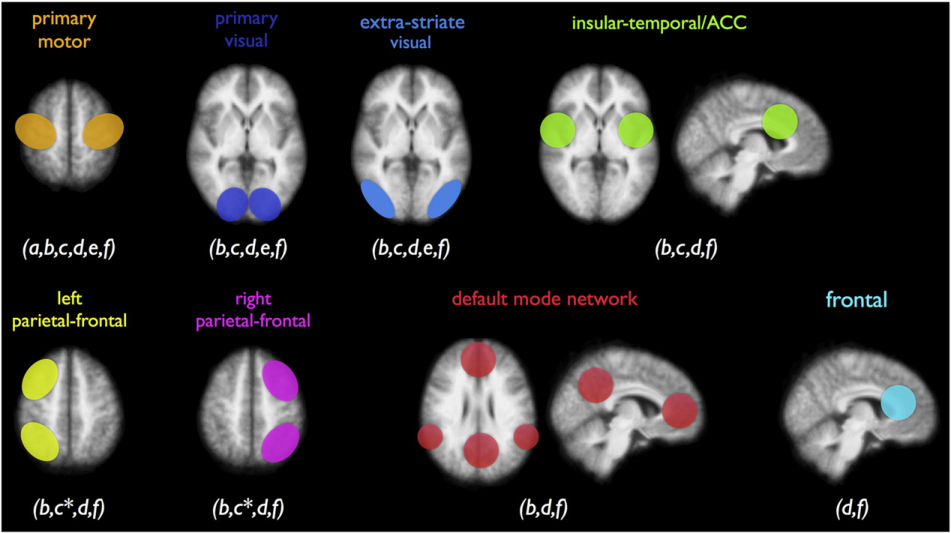
\includegraphics[width=1.0\textwidth]{images/vandenheuvel_networks.pdf}
\caption{Resting-state networks. A number of group resting-state studies have consistently reported the formation of functionally linked resting-state networks during rest. These studies, although all using different groups of subjects, different methods (e.g. seed, ICA or clustering) (Beckmann et al., 2005; Biswal et al., 1995; Damoiseaux et al., 2006; De Luca et al., 2006; Salvador et al., 2005a; Van den Heuvel et al., 2008a) and different types of MR acquisition protocols, show large overlap between their results, indicating the robust formation of functionally linked resting-state networks in the brain during rest. This figure shows the most consistent reported resting-state networks across these studies, including the primary sensorimotor network, the primary visual and extra-striate visual network, a network consisting of bilateral temporal/insular and anterior cingulate cortex regions, left and right lateralized networks consisting of superior parietal and superior frontal regions (*reported as one single network) and the so-called default mode network consisting of precuneus, medial frontal, inferior parietal cortical regions and medial temporal lobe. The figure illustrates resting-state networks reported by the following studies: (a) Biswal et al. (1995), (b) Beckmann et al. (2005), (c) De Luca et al. (2006), (d) Damoiseaux et al. (2006), (e) Salvador et al. (2005a), and (f) Van den Heuvel et al. (2008a).}
\label{fig:vandenheuvelnetworks}
\end{figure}
\todo{AGGIUNGERE COSE QUI E PARLARE DELLE VARIE NETWORKS CHE CI SONO}
% The analysis found 10 patterns with potential functional relevance, consisting of regions known to be involved in motor function, visual processing, executive functioning, auditory processing, memory, and the so-called default-mode network, each with BOLD signal changes up to 3\%. In general, areas with a high mean percentage BOLD signal are consistent and show the least variation around the mean

\section{Community detection in networks}
\label{sec:communitydetectioninnetworks}
% Most of the real-world networks exhibit a degree distribution that is not only globally, but also locally inhomogeneous, with high concentrations of edges within special groups of nodes, and low concentrations among such groups. This feature of real networks is called community structure. 
The process of grouping nodes in a graph to establish their common behavioral properties, is a popular technique that goes under the name of \emph{community detection}.
As the definition of community is not well stated (section ~\ref{sec:communities}), it is therefore important to have a quantitative way to evaluate the goodness of such clusterings.

The previously introduced concept of global criterion for the definition of communities can be also thought in terms of a fitness function defined over the clustering.
A \emph{quality function} is a function $\mathcal{Q}$ that given a clustering of a graph $\zeta$ returns a scalar number. Usually one identifies ``good'' clusterings with high scores of the quality function and ``bad'' clusterings with low scores. In this sense, is possible to rank partitions from bad to good, although is important to stress that the definition of ``good'' or ``bad'' is an \emph{ill-posed problem} as every quality function one designs puts the emphasis on some features of the community organization and perhaps not on others. 
Here and in the following sections, we strongly stress that the concept of quality function and community detection methods are separate as the first is a way to assess the goodness of a partition while the second relies on the definition of a quality function to design efficient algorithms and heuristics to find such good partitions.

One of the most important properties of a quality function is when it can be expressed as a sum over communities. Such quality functions are dubbed \emph{additive}: for a generic function of a cluster, or subgraph, $f(\zeta_i)$, an additive quality function specify the goodness of a clustering as sum of $f$ over the distinct communities as follows:
\begin{equation}\label{eq:additive_quality}
\mathcal{Q} = \sum \limits_{\zeta_c \in \zeta} f(\zeta_c).
\end{equation}
The majority of quality functions are additive, even if this requirement is not fundamental. In the next section we explore the properties of some of the most important additive quality functions that emerged from the literature of this decade.

\subsection{Spin glass based quality functions}
The simplest requirement of a quality function, is to put emphasis on intracluster edges and penalize intercluster edges. In this terms, local optima should correspond to partitions where the communities emerge as dense areas in the network loosely connected among them.
Here we present a general framework for the definition of suitable quality functions for community detection that meets these requirements.

This framework, introduced by Reichardt and Bornholdt~\cite{reichardt2006} is grounded in statistical mechanics, a branch of physics that studies the macroscopic and microscopic properties of systems of many interacting elements. Within this model, the problem of community detection is cast in terms of finding the \emph{ground state} of a spin glass, a model describing the behavior of large sets of interacting microscopic magnets.
Actually, the properties of spin glass models are subject of extremely intensive research in the last decades as their applications range from matter and nuclear physics to neural networks. Here we present only their salient application to community detection and refer the reader to cover the details of the model in other specialized books~\cite{mezard1990}.

A spin glass model starts from the definition of an Hamiltonian, a multi-variable scalar function that describe the total energy of the physical system with the configuration of its internal components. In our case, the internal components of the system are the nodes. The configuration of the system is then expressed by the community affiliation vector $\boldsymbol\sigma$, meaning that node $i$ stays in the community $\sigma_i$ (see~\ref{sec:clustering}).
The Hamiltonian used by Reichardt and Bornholdt (RB) counts four different contributions. The first two contributions act at intracluster level, positively weighing intracluster edges and negatively weighing intracluster non-edges with coefficients $a_{ij}$ and $b_{ij}$ respectively. The third and fourth contributions work on intercluster edges and non-edges, weighing them with factors $c_{ij}$ and $d_{ij}$. The general form of the RB model is then expressed by the following Hamiltonian:
\begin{align}\label{eq:hamiltonianspinglass}
\mathcal{H}^{\textrm{RB}}(\boldsymbol \sigma) = - \sum_{(i,j)\in V^2} & \left[ a_{ij} A_{ij} - b_{ij}(1-A_{ij}) \right] \delta(\sigma_i,\sigma_j) + \nonumber \\ &  \left[ (c_{ij} A_{ij} - d_{ij}(1-A_{ij}) \right] (1-\delta(\sigma_i,\sigma_j))
\end{align}
with the convention that lowest energy states correspond to best community assignments.
Rearranging Eq.\ref{eq:hamiltonianspinglass} and discarding the terms independent of the partition into a constant $H_0$, one then gets a simpler expression for $\mathcal{H}^{\textrm{RB}}(\sigma)$:
\begin{equation}\label{eq:rbspinglass}
\mathcal{H}^{\textrm{RB}}(\boldsymbol \sigma) = -H_0 - \sum \limits_{(i,j)\in V^2} \left[ \alpha_{ij} A_{ij} - \beta_{ij} \right] \delta(\sigma_i,\sigma_j)
\end{equation}
where the two parameters $\alpha_{ij}=a_{ij}+b_{ij}+c_{ij}+d_{ij}$ and $\beta_{ij}=b_{ij}+d_{ij}$ depend on the \emph{null model} one would like to compare with, i.e. the probability that an edge exists between $i$ and $j$ after random edge rewiring. Hence, a null model provides a mean to compare a specific set of features of a graph, with its randomized version that should specifically lack those features.

It's possible to express any quality function in the form of Eq.~\ref{eq:rbspinglass} as an additive quality function by setting $\alpha_{ij}=1$, $H_0=0$ and moving the summation indexes over the communities rather than over the pairs of nodes, as the sum is only over intracluster edges. The resulting Hamiltonian, expressed here as $\mathcal{H}^{\textrm{RB}}_{\textrm{reduced}}(\sigma)$, then reads:
\begin{equation}\label{eq:rbspinglass2}
\mathcal{H}^{\textrm{RB}}_{\textrm{reduced}}(\sigma) = -\sum_{(i,j) \in V^2} \left[ A_{ij} - \beta_{ij} \right] \delta(\sigma_i,\sigma_j) = - \sum \limits_{c}^C \left[ m_c - \left< m_c \right> \right].
\end{equation}
where $m_c=\sum_{ij}A_{ij}\delta(\sigma_i,c)\delta(c,\sigma_j)$ represents the number of links inside community labeled by $c$ and $\left <m_c \right >=\sum_{ij}\beta_{ij}\delta(\sigma_i,c)\delta(c,\sigma_j)$ is the expected number of links in community $c$ as prescribed by the null model $\beta_{ij}$\footnote{Here and for the rest of the work, we set $P_{ij}:=\beta_{ij}$ for agreement with more conventional notation of null models}. 
Among the additive quality functions that show up in the form of~\ref{eq:rbspinglass2}, the most important and popular is the \emph{Newman-Girvan's Modularity}.

\subsection{Newman-Girvan Modularity}\label{sec:newman_modularity}
Newman-Girvan Modularity (or simply Modularity)~\cite{newman2006}, denoted here and for the rest of the work by $Q^N$, is based on the idea that a network obtained by randomly reshuffling the original graph edges while keeping the same degrees sequence, should not display any community structure. 
An important consequence of such randomization is that any stub in this null model, dubbed ``configuration model'' is equally likely to be connected to any other~\cite{newman2010networks}. Thus, in absence of correlations, the probability that two nodes are connected is expressed by:
\begin{equation}\label{eq:configuration_model}
P_{ij} = \frac{k_i k_j}{2m}
\end{equation}
where $k_i$ and $k_j$ are the degrees of node $i$ and $j$. The ``configuration model''  is of great importance in network science as it assigns higher probability of link to nodes with high degrees, a feature that is compatible with most real world networks. 
We'll address the motivations of the configuration model in  details in section~\ref{sec:configuration_model}.

In terms of a spin glass model, Modularity measures the deviation from the observed intracluster density with respect to the expected intracluster density specified by the configuration model. Modularity is described in the form of~\ref{eq:rbspinglass2} but normalized by the number of edges in the graph, taking the form described in Eq.~\ref{eq:newmanmodularityspinglass}.
\begin{equation}\label{eq:newmanmodularityspinglass}
Q^N =  \frac{1}{2m} \sum_{ (i,j) \in V^2} \left[ A_{ij} - \frac{k_i k_j}{2m} \right] \delta(\sigma_i,\sigma_j),
\end{equation}
whereby optimal partitions have high values of $Q^N$. As already done in Eq.~\ref{eq:rbspinglass2}, Modularity can alternatively be expressed, as sum over communities of the difference of two terms:
\begin{equation}\label{eq:newmanmodularity}
Q^N = \sum_{c}^{|C|} \left[ \frac{m_c}{m} - \left( \frac{K_{\textrm{int}}(\mathcal{G}_c)}{2m} \right)^2 \right]
\end{equation}

Modularity takes values in the range $[-0.5,1]$, then a good partition should have $Q^N$ values close to unity, identifying groups with many more internal connections than expected at random. In contrast, a bad partition with $Q^N$ closer to zero should identify groups with no more internal connections than we expect at random.
In the next sections we will challenge this idea and show that this observation has lead to false statements, as a general phenomenon dubbed \emph{resolution limit}, heavily affects any quality function based on comparison with global null models. Specifically in the case of Newman's Modularity, the resolution limit hit hard.

\subsection{The configuration model}\label{sec:configuration_model}
A central property of the configuration model is the probability $P_{ij}$ of the occurrence of an edge between two specified vertices $i$ and $j$.
Let's consider anyone of the stubs that emerges from vertex $i$.
What is the probability that this stub is connected by an edge to any of the stubs of vertex $j$?
There are $2m$ stubs in total, or $2m - 1$ excluding the one connected to $i$ that we are currently looking at.
Of those $2m - 1$, exactly $k_j$ of them are attached to vertex $j$.
So, given that any stub in the network is equally likely to be connected to any other, the probability that our particular stub is connected to any of those around vertex $j$ is $k_j/(2m-1)$.
In absence of correlations, the probabilities that any two nodes $i$ and $j$ are connected to each other is given by the sum of the two independent probabilities for vertex $i$ and vertex $j$, defining the null model as:
\begin{equation}\label{eq:configuration_model_probability}
P_{ij} = \Pr \left ( a_{ij} | \{ k \} \right) = \Pr(k_i | \{ k \}) + \Pr(k_j | \{ k \})=\frac{k_i k_j}{2m}
\end{equation}

Although Modularity is most frequently applied to \emph{simple graphs} (see Fig.~\ref{fig:simple_unweighted_graph}), the configuration model implies that the randomization is carried over the space of \emph{loopy multigraphs} (Figure~\ref{fig:loopy_multigraph}).
The rewiring probability considers indeed that the stubs of nodes can be reconnected both to the same source vertex (self-loops) or added to already existing edges (multi-edges).
Consider for example the set of matchings on six stubs that form a triangle graph as illustrated in Figure~\ref{fig:configuration_model_stubs}. The configuration model chooses each distinct edge stubs labeling with equal probability. However, not only the first eight distinct reshuffled labellings are possible under configuration model (Fig.\ref{fig:reshuffle_simple_graphs}) but many other distinct matchings producing non-simple networks as shown in Figure~\ref{fig:reshuffle_loopy_multigraphs}.
In fact, the number of possible re-wirings that can be generated under the hypotheses of the configuration model, namely the presence of self-loops and multi-edges, is indicated by $\Omega_{CM}$ and can be computed by means of combinatorial arguments as:
\begin{equation}\label{eq:cm_possible_rewirings}
\Omega_{CM} = \binom{2m}{k_1,\ldots,k_n} = \frac{(2m)!}{\prod_i^n k_i!}.
\end{equation}
For the small triangle graph, this number is already very large: 90 different re-wirings are possible!
In practice though, the fraction of edges involved in either self-loops or multi-edges is vanishingly small in the large $n$ limit, and thus we may generally ignore them without much impact. 
Hence, the estimate of the probability of rewiring in Eq.~\ref{eq:configuration_model_probability} is only valid in large, sufficiently sparse graphs with a sufficiently bounded degree sequence.
Under these hypotheses the expected number of edges between two vertices in the space of simple graphs is asymptotically the same as the expectation in the space of stub-labeled loopy multigraphs, i.e. the one previously introduced for the definition of Modularity: $\mathbb{E}_s[a_{ij} |k] \approx k_i k_j /(2m)$, where the subscript $s$ denotes the space of simple graphs.

\begin{figure}[htb]\centering
\begin{subfigure}[t]{0.45\textwidth}\centering
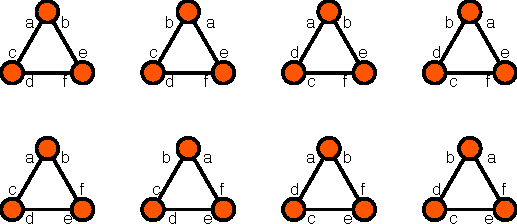
\includegraphics[height=2.4cm]{images/configuration_model_six_stubs.pdf}
\caption{}
\label{fig:reshuffle_simple_graphs}
\end{subfigure}
\begin{subfigure}[t]{0.45\textwidth}\centering
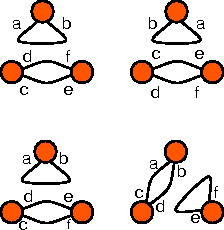
\includegraphics[height=2.4cm]{images/configuration_model_three_stubs.pdf}
\caption{}
\label{fig:reshuffle_loopy_multigraphs}
\end{subfigure}
\caption{Twelve of the ninety different possible rewirings of a triangle graph in the configuration model. In (a) only rewirings leading to simple graphs are considered. In (b) just four rewirings leading to loopy-multigraphs are shown.}
\label{fig:configuration_model_stubs}
\end{figure}
An approach that allows to get the right configuration model depending on the class of graph under exam, relies on the computational simulation of the correct rewiring probability by means of Markov Chain Monte Carlo algorithms, as proposed in~\cite{fosdick2016}.
In the remaining paragraphs, although flawed, we'll use the classic configuration model from Eq.~\ref{eq:configuration_model_probability} to be adherent to most of the brain networks literature, justified also by the vanishing effects of self-loops in large sparse networks. Nonetheless, we will illustrate many of the problems that the non critical use of Modularity with this null model has introduced.

\subsection{Other null models for Modularity}
Modularity identifies communities as subset of nodes whose internal fraction of edges deviates from the null configuration model on the same subset with the term $m_c/m > (K_c/2m)^2$.
Despite measuring deviation from a null model, Modularity does not take into account the statistical evidence associated with this deviation. For this reason, Modularity is not able to separate actual communities from those arising only from statistical fluctuations of the null model. Even worse, Modularity can find high-scoring partitions in fully random graphs~\cite{guimera2004} and in artificially built graphs with no community structure~\cite{kehagias2013}.

The configuration model is not the only possible null-model to use in spin-glass based quality functions. Different authors proposed several variants of Modularity~\cite{ronhovde2010,ronhovde2009,traag2011} with different null models.
The simplest variation of Modularity is the so-called ER Modularity~\cite{traag2015} that instead of the configuration model uses an Erd\H{o}s-Rényi random graph in which every edge appears with the same probability $p_{\textrm{ER}}$. The number of expected edges $\left< m_c \right>$ in a community of size $n_c$ is thus (in the space of simple graphs):
\begin{equation}
\left< m_c \right> = p_{\textrm{ER}}\binom{n_c}{2}.
\end{equation}
and plugging this null model into the RB model of Eq.~\ref{eq:rbspinglass2} we obtain the model:
\begin{equation}\label{eq:ermodularityrb}
\mathcal{H}^{ER} = -\sum \limits_c^C \left[\frac{m_c}{m}  - p_{\textrm{ER}}\binom{n_c}{2} \right].
\end{equation}
As the most similar ER graph of a given graph is the one that matches its density, the probability parameter $p_{\textrm{ER}}$ must be set equal to the original empirical graph density $\rho$. The so-called ER Modularity is derived by plugging the graph density in Eq.\ref{eq:ermodularityrb} and inverting its sign: 
\begin{equation}
Q^{ER} = \sum \limits_c^C \left[\frac{m_c}{m}  - \rho \binom{n_c}{2} \right].
\end{equation}
Under this model a group of nodes forms a community if its internal density is greater than the graph density $\rho$, on average.
Interestingly, from a machine learning perspective, all spin glass models quantify the discrepancy between observed and expected intramodule fraction of edges by means of a linear loss function. Among all the loss function, the linear is not the only possible and loss functions that take into account the relative size of clusters are possible.

\subsection{Comparing community structure in networks}
Some benchmark networks come with an annotated community structure representing the ground-truth assignment of nodes into communities, the annotations being made by experts in the field, like for example the karate-club network of Zachary~\cite{zachary1977} or the political blog network~\cite{adamic2005}.
Moreover, generative models of networks like the stochastic block model and its variants, the planted partition model and the LFR benchmark, have a known ground-truth community.
As the number of community detection methods increased over the years, also a quantitative way to assess their performance was requested.

A large number of functions for comparing similarities and differences between partitions of a network have been proposed in the past. They are used to provide quantitatively a number that tells how two partitions are similar.
Typically the result is normalized in the $[0,1]$ range, being towards $1$ for very similar clusterings and toward $0$ when mostly dissimilar. These metrics are adopted especially in the benchmarking of community detection methods, when the specific outcome of some algorithm is compared with a ground truth partition, usually a-priori determined.

The most well-grounded and performing metrics for the comparison of two community structures are rooted in information theory\cite{cover2006}.
The \emph{Normalized Mutual Information}~\cite{danon2005} and the \emph{Variation of Information}~\cite{meila2007} are the most widely used, despite it has been recently found that both of them suffer of systematic errors due to the finite size of the network \cite{zhang2015a}. In the rest of the discussions we ignore the limitation of finite size effects, by only working with relatively large networks.

Normalized Mutual Information (NMI) assumes that the clustering comparison is a problem of message decoding. Implicit in this, is the idea that if two partitions are similar, inferring one partition from the other needs very little information. 

Let us consider two generic partitions of a graph denoted by their clusterings $\zeta^x,\zeta^y$ with $c_x$ and $c_y$ communities respectively: $\zeta^x=\{\zeta^x_1,\ldots,\zeta^x_{c_x}\}$ and $\zeta^y=\{\zeta^y_1,\ldots,\zeta^y_{c_y}\}$.
The number of nodes in the $i$-th community of $\zeta^x$ is $n_i :=|\zeta^x_i|$ and the number of nodes in the $j$-th community of $\zeta^y$ is $n_j:=|\zeta^y_j|$. The two communities share a number of nodes $n_{ij}=| \zeta^x_i \cap \zeta^y_j|$.
Let us also consider the community assignments $\boldsymbol\sigma^x_i$ and $\boldsymbol\sigma^y_i$ for partitions $\zeta^x$ and $\zeta^y$ respectively; we treat the labels as values of two random variables $X$ and $Y$ with joint distribution $P(x,y)=P(X=x, Y=y) = n_{xy}/n$, which implies that $P(x)=P(X=x)=n_x^X/n$ and $P(y)=P(Y=y)=n_y^Y/n$.
The \emph{mutual information} between the two clusterings $\zeta^x,\zeta^y$ is then defined as 
\begin{equation}I(X,Y)=H(X) - H(X|Y)
\end{equation}
where $H(X)=-\sum_x p(x) \log p(x)$ is the Shannon entropy of $X$~\cite{cover2006}.
The mutual information itself is not very useful, because hierarchically splitting the clusters in $\zeta^x$ would produce no change in the prior $H(X|Y)$ and partitions with different hierarchies of the same clusters, would go unnoticed.
This observation led Danon~\cite{danon2005} to introduce normalized mutual information for clustering comparison as: 
\begin{equation}\label{eq:nmi}
\textrm{NMI}(X,Y) = \frac{2I(X,Y)}{H(X)+H(Y)}
\end{equation}
Explicitly, NMI is defined on top of the confusion matrix as:
\begin{equation}\label{eq:nmiexplicit}
\textrm{NMI} = \dfrac{2\sum \limits_{i=1}^{c_x} \sum \limits_{j=1}^{c_y} \frac{n_{ij}}{n} \log\left( \frac{n_{ij}n}{n_i n_j} \right)} {\left(-\sum \limits_{k=1}^{c_x} \frac{n_k}{n}\log\left(\frac{n_k}{n}\right) \right) + \left(-\sum \limits_{k=1}^{c_y} \frac{n_k}{n}\log\left(\frac{n_k}{n}\right) \right)}
\end{equation}

\begin{figure}
\centering
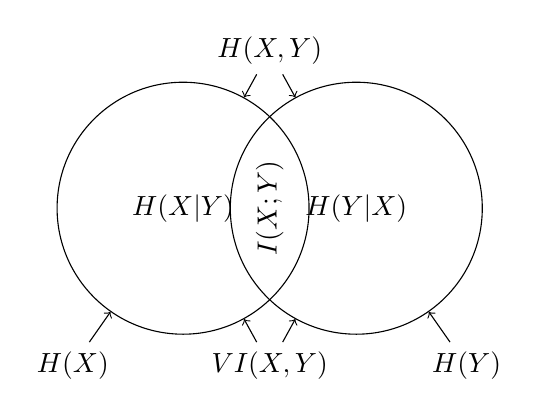
\begin{tikzpicture}
    \node[draw,circle,minimum size=3.2cm, inner sep=0cm] at (-1.1cm,0cm) (CL) {$H(X|Y)$};
    \node[draw,circle,minimum size=3.2cm, inner sep=0cm] at (1.1cm,0cm) (CR) {$H(Y|X)$};    
    \node[rotate=90] at (0cm,0cm) (IXY) {$I(X;Y)$};
    \node[] at (0cm,2cm) (HXY) {$H(X,Y)$};
    \node[] at (-2.5cm,-2cm) (HX) {$H(X)$};
    \node[] at (2.5cm,-2cm) (HY) {$H(Y)$};
    \node[] at (0cm,-2cm) (VI) {$VI(X,Y)$};
    \draw[->] (HX) -- (CL);
    \draw[->] (HY) -- (CR);
    \draw[->] (HXY) -- (CL);
    \draw[->] (HXY) -- (CR);
    \draw[->] (VI) -- (CL);
    \draw[->] (VI) -- (CR);
\end{tikzpicture}
\caption{Venn diagram representation of the important quantities used to treat the clustering comparison problem in terms of information theory. The two circles are the entropies of variables $X$ and $Y$. The mutual information $H(X;Y)$ is the intersection of the information in $X$ with the information in $Y$. The Variation of information is equal to $VI(X;Y)=H(X|Y)+H(Y|X)=H(X)+H(Y)-2I(X;Y)$ because $I(X;Y)$ is counted twice.}
\end{figure}

Meila proposed another measure based on entropy, Variation of Information (VI)~\cite{meila2007}. VI measures how much knowing the cluster assignment for an item in clustering $X$ reduces the uncertainty about the item's cluster in clustering $Y$. Is defined as:
\begin{equation}\label{eq:vi}
\textrm{VI}(X,Y) = H(X|Y) + H(Y|X)
\end{equation}
and it has the desirable property that, being a proper distance, it defines a metric on the space of the partitions.
Variation of information is also a local measure, i. e. the similarity of partitions differing only in a small portion of a graph depends on the differences of the clusters in that region, and not on the partition of the rest of the graph.
As noted by Karrer \cite{karrer2008} VI is upper-bounded by a $\log(n)$ factor, so a simple normalization brings it in the $[0,1]$ range. 
Importantly, VI is zero for maximally equal partitions and $1$ for mostly dissimilar, inversely to NMI.

It's worth noting that the majority of the aforementioned metrics do not take in consideration comparison of pairs of communities between two partitions, but they insist on finding overall similarity to summarize it in a single scalar.

% It is possible though to study partitioning on a community-wise basis by explicitly enumerating all the similarity between groups of nodes of two different partitions.

% Let's assume we have two different clusterings $\zeta^x,\zeta^y$ obtained from two different runs of some non-deterministic community detection algorithm. For two communities $c_i \in \zeta_1, c_j \in \zeta_2$, with $1\leq i \leq |\zeta_1|$,$1\leq j \leq |\zeta_2|$ then the cluster homogeneity is defined as:

% \begin{align}
% \Pr(\textrm{overlap}) = \frac{\binom{|c_j|}{|c_i \cap c_j|}\binom{N-|c_j|}{|c_i|-|c_i \cap c_j|}}{\binom{N}{|c_i|}}
% \end{align}
% %
% \todo{fix discorso cluster homogeneity}

\section{Resolution limit}\label{sec:resolutionlimit}
Modularity attracted a lot of attention over the years as it  became the tool of election to inspect the community structure of networks.
On one side, the wide use of Modularity, led many researchers to gain interest in complex networks, with results in sociology~\cite{li2008tag}, bioinformatics~\cite{saracc2012topology} and ICT~\cite{java2007we,leskovec2007dynamics}, just to mention a few, but on the other side it offered a fallacious view on the community detection problem.
Indeed, although simple in many sense, Modularity optimization was hiding a problem that heavily limits its use in real world networks.

In 2007, a seminal article by Fortunato and Barthelemy~\cite{fortunato2007} did a thoroughly analysis of Modularity.
Their work showed the inability of Modularity to correctly identify communities that are smaller than a certain scale, determined by the square root of the number of edges. They dubbed this general phenomenon \emph{resolution limit}.
To illustrate what is meant by the resolution limit, here we follow the example of Fortunato and Barthelemy, with some obvious notational change.

Let us consider a toy network, $G=(V,E)$ that is composed of three subnetworks, as shown in~\ref{fig:figure_1_barthelemy}A.
The first subnetwork, a subgraph $G_0$ with $n_0$ nodes and $m_0$ edges is connected to two cliques, $G_1$ and $G_2$ by $m_{01}$ and $m_{02}$ links respectively. The two cliques are also connected by a number of $m_{12}$ links as shown in Figure~\ref{fig:figure_1_barthelemy}.
While $G_1$ and $G_2$, are complete subgraphs and are expected to be modules by construction, $G_0$ may consist of many communities. Maximum Modularity partitions then, should identify $G_1$ and $G_2$ as communities, independently from $G_0$.
To be more specific, let the partition where the two cliques are separated be denoted by $A$, with Modularity value $Q_A$. On the other hand, the partition where the two cliques are merged into a single community is denoted by $B$, with Modularity value $Q_B$.
To ease the calculations, we indicate the number of links $m_{12}$ as functions of $m_1$ and $m_2$, such that $m_{12}=a_{1}$, $m_1=a_2 m_2$, $m_{01}=b_1 m_1$ and $m_{02}=b_2 m_2$ with $a_1,a_2,b_1,b_2 \geq 0$.

As Modularity is a sum over the modules, and the module $G_0$ has the same Modularity $Q_0$ in both partitions, we are interested in studying the difference $\Delta Q = Q_{A} - Q_{B}$. After some simple algebraic manipulations it results:
\begin{equation} \label{eq:resolution_limit_delta}
\Delta Q = \frac{2 m a_1 m_1 - (a_1+b_1+2)(a_2+b_2+2)m_1 m_2}{2m^2}
\end{equation}
Specifically, we want to check when $\Delta Q > 0$, i.e. when the partition $A$ has a higher Modularity than partition $B$. This condition is verified as long as
\begin{equation}
m_2 < \frac{2m a_1}{(a_1+b_1+2)(a_2+b_2+2)}.
\end{equation}
In the case where $a_1=a_2=0$, there are no links between $G_1$ and $G_2$ and the condition is satisfied. When instead the two subgraphs are connected ($m_{12} \neq 0$), it happens that at some values of $m_1$ and $m_2$, the partition where the two modules are merged is preferred, i.e. $\Delta Q <0$. This means that when maximizing $Q^N$ on a network, is possible to miss some important structures, if they are too small.
More specifically, if the two modules have the same size and one sets $a_1=a_2=b_1=b_2=1/m$, is easy to check that Eq.~\ref{eq:resolution_limit_delta} is not satisfied if the number of links in the modules $m_c$, is lower than the square root of the total number of links in the network:
\begin{equation}
m_c < \sqrt{\frac{m}{2}}.
\end{equation}

To make this example more concrete we studied numerically a toy network where the three subgraphs take a precise form.
For the sake of illustration, we have defined $G_1$ and $G_2$ as two identical cliques of $5$ nodes connected to $G_0$ by a single edge ($m_{01}=m_{02}=1$) and to each other by $m_{12}$ edges.
The module $G_0$ was defined as a clique of variable size with a number of edges ranging from 45 to 2775. We then computed the numerical difference $\Delta Q$ and plotted it as a function of the number of edges $m_0$ in the $G_0$ clique. The onset of the resolution limit occurs when $\Delta Q$ changes sign and becomes negative for increasing values of $m_0$.
For $m_{12}=1$, i.e. when the two cliques $G_1$ ad $G_2$ were connected by only one edge (red curve), $Q$ showed this sign inversion for $m_0 \approx 200$ (Figure \ref{fig:figure_1_barthelemy}B).
With increasing number of intercluster edges $m_{12}$, the resolution limit appeared for smaller and smaller values of $m_0$, eventually leading to $\Delta Q$ values that were always negative, i.e. the two cliques $G_1$ and $G_2$ were always merged by Modularity optimization.


\begin{figure}[htb!]
\centering
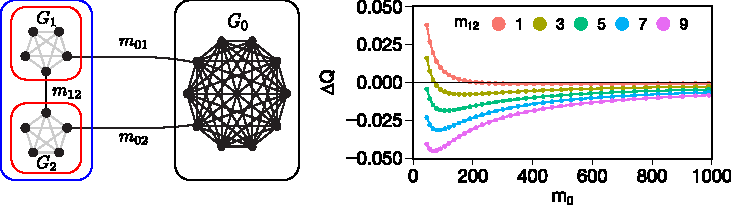
\includegraphics[width=1\textwidth]{images/barthelemy_modularity.pdf}
\caption{Analysis of the onset of the resolution limit for Modularity in a model graph (A) consisting of two cliques, $G_1$ and $G_2$, and a size-varying components $G_0$. The red line indicates the partition $A$, with $G_1$ and $G_2$ as different modules, and the blue line the partition $B$, with $G_1$ and $G_2$ merged into a single module. The graph (B) shows the difference in Modularity for increasing number of edges in $G_0$.}
\label{fig:figure_1_barthelemy}
\end{figure}

An even more striking example of how the resolution limit affects Modularity is when looking at the optimal partition of a synthetic lattice graph, known as ``ring of cliques'', a network made out of identical cliques, connected in a ring-like structure by single links, as shown in Figure~\ref{fig:traag_ring_of_cliques}. 

\begin{figure}[htb!]
\centering
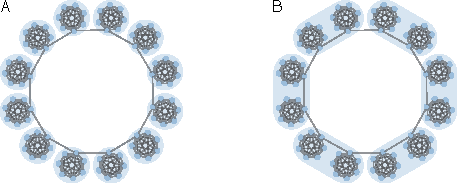
\includegraphics[width=1\textwidth]{images/traag_ring_of_cliques.pdf}
\caption{In this toy network, the intracommunity density is the highest possible, while the intercommunity density is the lowest to keep the network connected. The correct community structure is clearly the one on left (A), but Modularity values is higher for the partition on the right (B), where pairs of cliques are coalesced into separated communities.}
\label{fig:traag_ring_of_cliques}
\end{figure}
If the number of cliques is large enough (they are more than $\sqrt{m}$), Modularity optimization leads to a partition where the cliques are combined into groups of two or more. This phenomenon can be observed already when considering a ring of 30 cliques made of 5 nodes, when the optimal Modularity partition combines cliques in pairs.
Yet extending the number of cliques, Modularity may merge cliques into groups of three, fours etc.

\subsection{Resolution parameter}
Fixes have been proposed to circumvent the resolution limit, including the introduction of a tunable parameter that enables analysis of the network at an adjustable resolution level~\cite{reichardt2006,ronhovde2010,yeo2011}.

In this sense, the most common tuning to the Modularity quality function is the one that takes in consideration a \emph{resolution parameter}.
From the definition of $Q^N$ is evident that is possible to tune the size of the detected modules by multiplication of the configuration null model by a constant factor $\gamma_{N} \in [0,1]$, resulting in a modified modularity $Q^N(\gamma)$:
\begin{equation}
Q^N(\sigma,\gamma) = \sum_c^C \left[ \frac{m_c}{m} - \gamma_{N} \left( \frac{K_c}{2m}\right)^2 \right].
\end{equation}
However, exact specification of $\gamma_{N}$ requires prior knowledge of the expected size of the communities.
Moreover, it has been shown~\cite{lancichinetti2011} that an adjustable resolution parameter may reduce the tendency to merge small clusters, but only at the cost of unduly splitting large clusters. 
Indeed this is due to two opposite coexisting effects: the tendency to merge small subgraphs, which dominates when the resolution is low and the tendency to split large subgraphs, which dominates when the resolution is high.

In benchmark networks with heterogeneous distributions of cluster sizes, the simultaneous elimination of both biases is not possible and multi-resolution modularity is not capable to recover the planted community structure even in graphs where the ground-truth structure is evident.
Therefore, adjustment of the resolution parameter is an attempt to balance these two biases, but multi-resolution methods fail to recover community structures comprising heterogeneous distributions of cluster sizes~\cite{lancichinetti2011}. 

In another attempt to better tolerate the resolution limit, scholars applied appropriate techniques of edge re-weighting~\cite{berry2011} to enhance communities prior to Modularity maximization.
Although this technique proved able to better tolerate the detrimental effect of the resolution limit, it only shifted the scale of the problem.
After all, real-world networks are characterized by the coexistence of clusters of very different sizes, therefore no single parameter can adapt to the variety of network topologies observed in nature.

\subsection{Resolution-limit free quality functions and the Constant Potts Model}
In an attempt to quantitatively characterize the resolution limit, Traag et al.~\cite{traag2011} proposed a rigorous definition of \emph{resolution-limit-free} graph partitioning.

A quality function is resolution-limit-free if, given an optimal partition $\zeta$ of a graph $G$, any module $\zeta_i$ is also optimal for the graph induced by the nodes in $\zeta_i$.
In other words, each community of the optimal partition is not split by optimization of the quality function applied to the subgraph induced by the nodes in the community.
Hence, each community does not depend on the rest of the network and is both locally and globally optimal.
Then, in order to design such resolution-limit-free quality function, Traag took a spin glass model, with a null model specified by constant quantity $\gamma_{\textrm{CPM}}$~\cite{traag2011} and dubbed it \emph{Constant Potts Model}.

The \emph{Constant Potts Model} (CPM) identifies community as subset of nodes whose internal density $\rho_c$ is bigger than the overall graph density multiplied by a factor $\gamma_{\textrm{CPM}}$ that defines the typical scale of the communities. In the framework of Reichardt and Bornholdt, the CPM model has the following Hamiltonian: 
\begin{equation}\label{eq:cpm_hamiltonian}
H(\sigma)^{\textrm{CPM}} = - \sum \limits_{(i,j) \in V^2} \left[ a_{ij} - \rho \gamma_{\textrm{CPM}} \right] \delta(\sigma_i,\sigma_j),
\end{equation}
that once reworked in an additive quality function, results in the form of Eq.~\ref{eq:cpm_hamiltonian} 
\begin{equation}\label{eq:cpm_ermodel}
Q^{\textrm{CPM}} = \sum \limits_c^{|C|} \left[m_c - \gamma_{\textrm{CPM}} n_c^2 \right] 
\end{equation}
In other words, the model tries to maximize the number of internal edges while at the same time keeping relatively small communities. The parameter $\gamma_{\textrm{CPM}}$ balances these two imperatives; indeed it acts as the inner and outer edge density threshold.
In the CPM settings is better to split two communities $r$ and $s$ if $\gamma_{CPM}$ exceeds the inter-community density $m_{r,s}/(2n_r n_s)$.

Unfortunately, the operation of tuning the resolution parameter, both in the CPM model as well as in other similar models, is difficult and no largely accepted method exists, making all the models based on a resolution parameter, scarcely used in practical applications.

\subsection{Effects of resolution limit}
In the context of brain networks, the resolution limit first highlighted by Fortunato and Barthelemy may be particularly critical for the analysis of brain connectivity networks, as it may unduly merge modules that are too small, therefore hampering the ability to highlight regions of functional segregation from the rest.
By way of example, certain functional processes, like color vision, have been described as anatomically localized~\cite{zeki1998}, while others, like working memory, have been proposed to involve more globally integrated processing systems~\cite{baddeley2003}.

Hence, we may expect the brain modular structure to comprise heterogeneously distributed communities. Whether the relatively uniform modular structure of brain connectivity, highlighted by Newman's Modularity and other community detection methods in many studies, reflects the true architecture of the brain organization or is the result of the resolution limit is still unclear.
Hierarchical approaches have shown that large modules can be further subdivided, indicating that connectivity networks show structure at different spatial scales~\cite{meunier2009}.
However, these findings do not provide information on the optimal partition of the network, i.e. the optimal cut through the dendrogram representing connectivity at the different scales.

Thus, the resolution limit is a critical shortcoming for the study of brain networks and is likely to have affected many of the studies reported in the literature. The limitation on the number of detected modules in brain networks is evident in studies where typically four or five communities of the same size are detected in humans, as in Crossley et al.~\cite{crossley2013a}, Meunier et al.~\cite{meunier2009a,meunier2010}, Fair et al.~\cite{fair2009} or also in mouse models~\cite{schwarz2008}. To this end, an optimization method that does not suffer from the resolution limit would be needed.

It's also very important to stress that comparing the Modularity value $Q^N$ across different networks obtained in different studies, with possibly different number of nodes or different densities is an erroneous practice although $Q^N$ is normalized in the range $[0,1]$. As shown by a number of studies~\cite{good2009,kehagias2013,radicchi2010}, even in graphs which do have a natural community structure, high modularity values can be achieved by partitions which do not respect this natural structure. Hence, the Modularity value is only a numerical indication of the current status of optimization of the detected community structure on a specific graph and should never be confronted across different networks.


%%%%%%%%%%%%%%%%%%%%%%%%%%%%%%%%%%%%%%%%%%%%%
%%%%%%%%%%%%%% DEGENERACY %%%%%%%%%%%%%%%%%%%
%%%%%%%%%%%%%%%%%%%%%%%%%%%%%%%%%%%%%%%%%%%%%
\section{Degeneracy}\label{sec:degeneracy}
The differences in Modularity between optimal and suboptimal partitions can be very small, as observed in Figure~\ref{fig:figure_1_barthelemy}B, where $\Delta Q$ between the two partitions with splitted or merged cliques, remains close to zero for a large range of $m_0$ especially at $m_{12}=1$.
Indeed, even in the case where it would not be beneficial for Modularity to merge two modules, i.e $\Delta Q <0$, this difference can be made arbitrarily close to zero.

The total number of different partitions in a graph is the Bell number $B_n$~\cite{stanley1997} and it grows faster than exponentially in $n$, therefore a combinatorially large number of sub-optimal partitions exist around the global optimum. These partitions may be very close in terms of Modularity to the optimum but radically different in terms of similarity.
Thus, counter-intuitively, when the network becomes more modular, the globally optimal partitions becomes harder to find among the growing number of suboptimal but competitive alternatives.

This consideration explains the empirical observation that nearly-optimal solution tend to group into high-modularity plateaus, although they may differ substantially~\cite{good2009}. This phenomenon, dubbed \emph{degeneracy} affects Newman's Modularity and probably many other spin-glass based quality functions.
As a matter of example, the variation in Modularity for merging a pair of adjacent cliques in the ring of cliques graph shown in Figure~\ref{fig:traag_ring_of_cliques}, is given by:
\begin{equation}\label{eq:modularity_difference_ring_clique}
\Delta Q = \frac{1}{r\left(\binom{n_r}{2}+1\right)}-2r^{-2}
\end{equation}
where $r$ is the number of cliques and $n_r$ the number of nodes in each clique.
In the large $r$ limit, the difference in Eq.~\ref{eq:modularity_difference_ring_clique} tends to a small negative value, indicating that a solution where the cliques are merged, may have a Modularity very close to the optimum. Indeed, already for $r=20$ cliques, $\Delta Q \approx 5\times 10^{-3}$, making all the suboptimal partitions where cliques are merged, very close to the optimal solution.

To make this argument more intuitive, we extrapolated a visually appealing form of the complex landscape of partitions' Modularity for a ring of cliques network. We sampled the configuration space of the partitions of a ring of clique network through a Montecarlo procedure and annotated the corresponding values of Modularity for every partition as in~\cite{good2009}.
We then built a similarity matrix between all sampled partitions and embedded it into a three-dimensional space maintaining similarity relations between partition following a Curvilinear Components Analysis (CCA).
In the embedded manifold, two partitions are close if they are similar and the z-axis encodes the quality function.
An highly degenerate plateu can be observed in~\ref{fig:degeneracylandscape} whereby different solutions with high values of Modularity stay in the same neighborhood.

\begin{figure}[htb!]
\centering
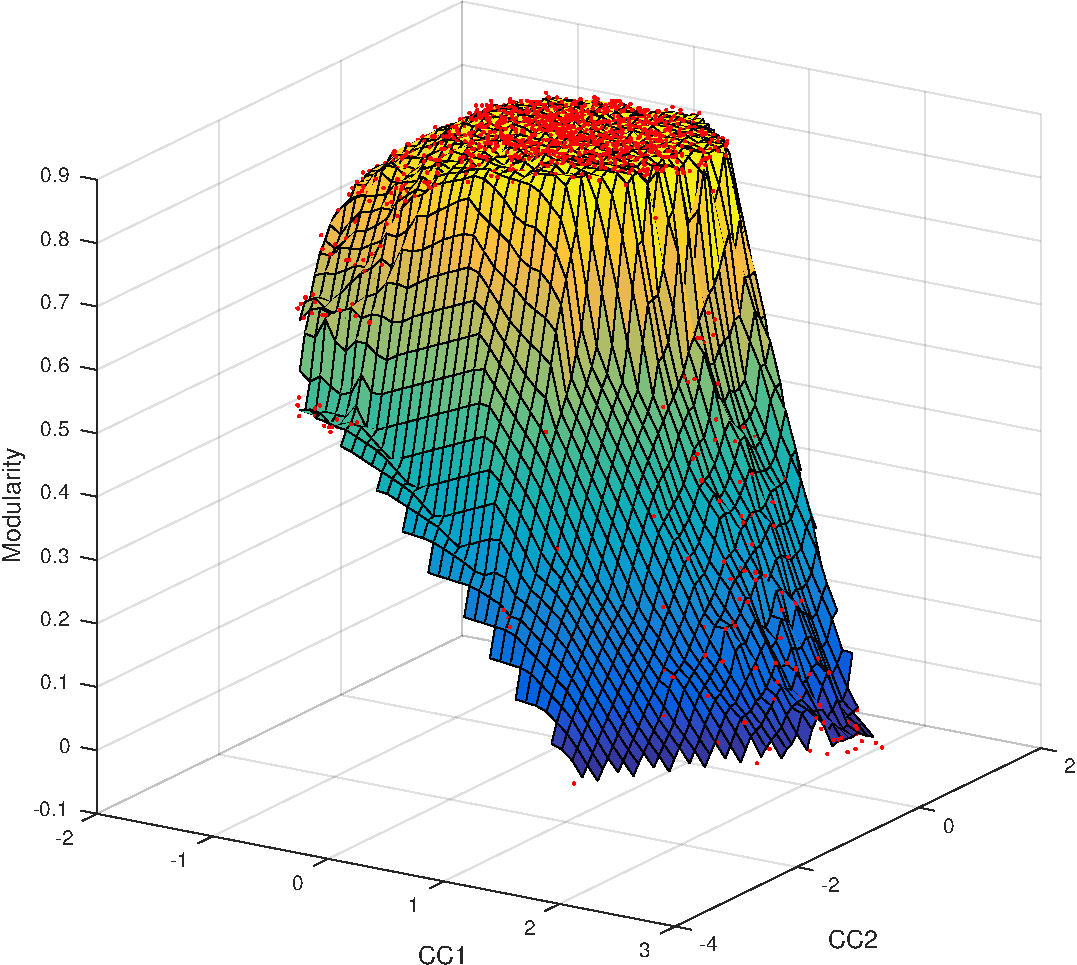
\includegraphics[width=0.75\textwidth]{images/degeneracy_modularity.pdf}
\caption{Degeneracy landscape for Newman's Modularity in a ring of cliques with $r=24$ cliques of $n_r=5$ nodes. The axes CC1 and CC2 are complicated functions of the original partition space computed as to maintain the distance relation between points and their scale is unimportant.}
\label{fig:degeneracylandscape}
\end{figure}

Any quality function suffering degeneracy of solutions, should display an embedded landscape with a plateau of optimal partitions, like the one shown in Figure~\ref{fig:degeneracylandscape}, while instead in the case of the existence of a net global optimum, a sharper peak should be exhibited.
We'll see that recasting the problem of community detection in terms of probability theory, will help in the definition of a quality function showing convex behavior and uniqueness of the optimum solution.

\section{Consensus clustering}
The issue of degeneracy is not only affecting Newman's Modularity $Q^N$ but other quality functions as well.
In this respect, it's clear that choosing the partition with the highest quality value isn't meaningful and a choice that consider all the good partitions at the plateau is desired. 
An optimal partition of the network can then be expressed as a \emph{median} of the solutions over the optimal plateau.
This approach known as \emph{consensus clustering} is advantageous to combine strengths and weakness of found partitions, whereby some local effects of noise during optimization are averaged over a large set of solutions.
Such approach for consensus clustering is typically based on a meta-algorithm rather than a proper community detection method. Indeed, given a community detection method, consensus clustering forms an ensemble of optimal solutions from which an association matrix $\mathcal{A}$ is computed, where edges are proportional to the probability that two nodes are connected in the same community.
Consensus communities are then obtained clustering iteratively the thresholded  association matrix. The choice of the threshold that makes the association matrix sparser~\cite{lancichinetti2012} is dictated by the properties of the chosen method of community detection itself. Typically with a smartly chosen threshold, consensus clustering converges in a few iterations. The pseudo-code illustrated in Alg.~\ref{alg:consensus_clustering} illustrates all the steps of consensus clustering.

\begin{Algorithm}[htb!]
\begin{codebox}
\Procname{\proc{ConsensusClustering}(a graph $G$, a community detection method)}
\li Apply community detection on $G$ for $n_p$ times, yielding $n_p$ different partitions.
\li Compute the consensus (association) matrix $\mathcal{A}$ where $\mathcal{A}_{ij}$ is the probability \\that vertex $i$ and $j$ are assigned in the same community over $n_p$ partitions.
\li Threshold the association matrix $\mathcal{A}$ with a parameter $\tau$.
\li Apply community detection on $\mathcal{A}$ for $n_p$ times to yield $n_p$ partitions.
\li If $\mathcal{A}$ is block diagonal (all partitions are equal) stop, else return to 1.
\end{codebox}
\caption{Pseudocode for the implementation of consensus clustering.}
\label{alg:consensus_clustering}
\end{Algorithm}

\section{The bias of the null model for Modularity}
Functional connectivity networks are typically measured as the Pearson correlation of time series of BOLD signals from different areas of the brain. When trying to extrapolate an optimal community assignment on such correlation matrix though, the null model of Modularity is not appropriate. As shown in a paper by MacMahon~\cite{macmahon2015}, indeed the configuration model introduces a systematic bias as it is not consistent with the definition of Pearson correlation.
Ideally, the Modular structure in a full correlation matrix (a correlation matrix with all nonzero entries) should reflect a balance between positively and negatively correlated units. Specifically, correlation communities should be internally positively correlated while externally negatively correlated. The null model proposed by MacMahon and Garlaschelli~\cite{macmahon2015} redefines the null model of Modularity to take into consideration such desired property. Thanks to the \emph{random matrix theory} the bulk of signal due to the global mode, a large scale oscillation that positively correlates all areas, is removed


 \todo{citare articolo garlaschelli?}